% Created 2017-03-27 Mon 16:57
% Intended LaTeX compiler: pdflatex
\documentclass[presentation]{beamer}
\usepackage[utf8]{inputenc}
\usepackage[T1]{fontenc}
\usepackage{graphicx}
\usepackage{grffile}
\usepackage{longtable}
\usepackage{wrapfig}
\usepackage{rotating}
\usepackage[normalem]{ulem}
\usepackage{amsmath}
\usepackage{textcomp}
\usepackage{amssymb}
\usepackage{capt-of}
\usepackage{hyperref}
\usetheme{CambridgeUS}
\usecolortheme{beaver}
\setcounter{secnumdepth}{1}
\author{Zheng Tian}
\date{}
\title{Lecture 7: Hypothesis Test  of Linear Regression with a Single Regressor}
\hypersetup{
 pdfauthor={Zheng Tian},
 pdftitle={Lecture 7: Hypothesis Test  of Linear Regression with a Single Regressor},
 pdfkeywords={},
 pdfsubject={},
 pdfcreator={Emacs 25.1.1 (Org mode 9.0.3)}, 
 pdflang={English}}
\begin{document}

\maketitle
\begin{frame}{Outline}
\setcounter{tocdepth}{1}
\tableofcontents
\end{frame}



\section{Testing Hypotheses about One of the Regression Coefficients}
\label{sec:orgdcd2f82}

\begin{frame}[label={sec:org1d89d22}]{The question after estimation}
\begin{equation}
\label{eq:testscr-str-1e}
\widehat{TestScore} = 698.93 - 2.28 \times STR
\end{equation}

\begin{itemize}
\item Now the question faced by the superintendent of the California
elementary school districts is whether the estimated coefficient on
\emph{STR} is valid.

\item In the terminology of statistics, his question is
whether \(\beta_1\) is statistically significantly different from
zero.
\end{itemize}
\end{frame}

\begin{frame}[label={sec:orgb37ff80}]{Step 1: set up the two-sided hypothesis}
\[ H_0: \beta_1 = \beta_{1,0}, H_1: \beta_1 \neq \beta_{1,0} \]
\end{frame}

\begin{frame}[label={sec:orgead7e54}]{Step 2: Compute the t-statistic}
\begin{itemize}
\item The general form of the t-statistic is
\begin{equation}
\label{eq:general-t}
t = \frac{\text{estimator} - \text{hypothesized value}}{\text{standard error of the estimator}}
\end{equation}

\item The t-statistics for testing \(\beta_1\) is
\begin{equation}
\label{eq:t-stat-b1}
t = \frac{\hat{\beta}_1 - \beta_{1,0}}{SE(\hat{\beta}_1)}
\end{equation}
\end{itemize}
\end{frame}

\begin{frame}[label={sec:orgb5465a5}]{The standard error of \(\hat{\beta}_1\) is calculated as}
\begin{equation}
\label{eq:se-b-1}
SE(\hat{\beta}_1) = \sqrt{\hat{\sigma}^2_{\hat{\beta}_1}}
\end{equation}
where
\begin{equation}
\label{eq:sigma-b-1}
\hat{\sigma}^2_{\hat{\beta}_1} = \frac{1}{n} \frac{\frac{1}{n-2} \sum_{i=1}^n (X_i - \bar{X})^2 \hat{u}^2_i}{\left[ \frac{1}{n} \sum_{i=1}^n (X_i - \bar{X})^2 \right]^2}
\end{equation}
\end{frame}

\begin{frame}[label={sec:org5171fb1}]{How to understand the equation for \(\hat{\sigma}^2_{\hat{\beta}_1}\)}
\begin{itemize}
\item \(\hat{\sigma}^2_{\hat{\beta}_1}\) is the estimator of the variance of
\(\hat{\beta}_1\), i.e., \(\mathrm{Var}(\hat{\beta}_1)\).

\item The variance of \(\hat{\beta}_1\) is 
\[ \sigma^2_{\hat{\beta}_1} = \frac{1}{n} \frac{\mathrm{Var}\left( (X_i - \mu_X)u_i \right)}{\left( \mathrm{Var}(X_i) \right)^2} \]

\item The denominator in \(\hat{\sigma}^2_{\hat{\beta}_1}\) is a consistent
estimator of \(\mathrm{Var}(X_i)^2\).

\item The numerator in \(\hat{\sigma}^2_{\hat{\beta}_1}\) is a consistent
estimator of \(\mathrm{Var}((X_i - \mu_X)u_i)\).

\item The standard error computed as \(\hat{\sigma}^2_{\hat{\beta}_1}\) is
the \alert{heteroskedasticity-robust standard error}.
\end{itemize}
\end{frame}

\begin{frame}[label={sec:orge884190}]{Step 3: compute the p-value}
\begin{itemize}
\item The p-value is the probability of observing a value of \(\hat{\beta}_1\)
at least as different from \(\beta_{1,0}\) as the estimate actually
computed (\(\hat{\beta}^{act}_1\)), assuming that the null hypothesis is
correct. 

\begin{equation*}
\begin{split}
p\text{-value} &= \mathrm{Pr}_{H_0} \left( | \hat{\beta}_1 - \beta_{1,0} | > | \hat{\beta}^{act}_1 - \beta_{1,0} | \right) \\
&= \mathrm{Pr}_{H_0} \left( \left| \frac{\hat{\beta}_1 - \beta_{1,0}}{SE(\hat{\beta}_1)} \right| > \left| \frac{\hat{\beta}^{act}_1 - \beta_{1,0}}{SE(\hat{\beta}_1)} \right| \right) \\
&= \mathrm{Pr}_{H_0} \left( |t| > |t^{act}| \right)
\end{split}
\end{equation*}
\end{itemize}
\end{frame}

\begin{frame}[label={sec:org01dd82b}]{Step 3: compute the p-value (cont'd)}
\begin{itemize}
\item With a large sample, the t statistic is approximately distributed as
a standard normal random variable. Therefore, we can compute 
\[p\text{-value} = \mathrm{Pr}\left(|t| > |t^{act}|
  \right) = 2 \Phi(-|t^{act}|)\]
where \(\Phi(\cdot)\) is the c.d.f. of the standard normal
distribution.

\item The null hypothesis is rejected at the 5\% significance level if the
\(p\text{-value} < 0.05\) or, equivalently, \(|t^{act}| > 1.96\).
\end{itemize}
\end{frame}

\begin{frame}[label={sec:org210bcff}]{Application to test scores}
\begin{equation*}
\widehat{TestScore} = \underset{\displaystyle (10.4)}{698.9} - \underset{\displaystyle (0.52)}{2.28} \times STR,\; R^2 = 0.051,\; SER = 1.86
\end{equation*}

\begin{itemize}
\item The \alert{heteroskedasticity-robust} standard errors are reported in the
parentheses.

\item The null hypothesis against the alternative one as
\[ H_0: \beta_1 = 0, H_1: \beta_1 \neq 0 \]

\item The t-statistics is
\[ t = \frac{\hat{\beta}_1}{SE(\hat{\beta}_1)} = \frac{-2.28}{0.52}
  = -4.38 < -1.96 \]

\item The p-value associated with \(t^{act} = -4.38\) is approximately
0.00001, which is far less than 0.05. So we reject the null
hypothesis.
\end{itemize}
\end{frame}

\begin{frame}[label={sec:org2299bf5}]{Rejecting the null hypothesis}
\begin{figure}[htbp]
\centering
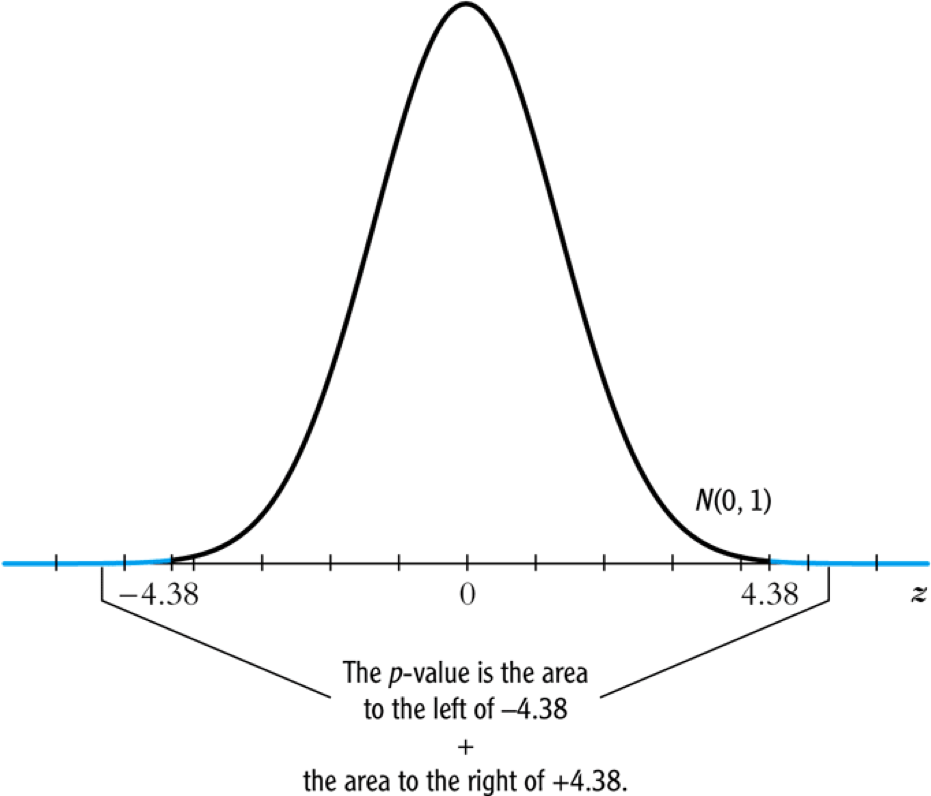
\includegraphics[width=0.7\textwidth]{figure/fig-5-1.png}
\caption{\label{fig:org0cec173}
Calculating the p-value of a two-sided test when \(t^{act}=-4.38\)}
\end{figure}
\end{frame}

\begin{frame}[label={sec:org258748f}]{The one-sided hypotheses}
\begin{itemize}
\item In some cases, it is appropriate to use a one-sided hypothesis
test. For example, the superintendent of the California school
districts want to know whether an increase in class sizes has a
negative effect on test scores, that is, \(\beta_1 < 0\).

\item For such a test, we can set up the null hypothesis and the one-sided
alternative hypothesis as

\[ H_0: \beta_1 = \beta_{1,0} \text{ vs. } H_1: \beta_1 < \beta_{1,0} \]
\end{itemize}
\end{frame}

\begin{frame}[label={sec:org783e35d}]{The one-sided left-tail test}
\begin{itemize}
\item The t-statistic is the same as in a two-sided test
\[ t = \frac{\hat{\beta}_1 - \beta_{1,0}}{SE(\hat{\beta}_1)} \]

\item Since we test \(\beta_1 < \beta_{1,0}\), if this is true, the
t-statistics should be statistically significantly less than zero.

\item The p-value is computed as \(\mathrm{Pr}(t < t^{act}) = \Phi(t^{act})\).

\item The null hypothesis is rejected at the 5\% significance level when
\(\text{p-value} < 0.05\) or \(t^{act} < -1.645\).

\item In the application of test scores, the t-statistics is -4.38, which
is less than -1.645 and -2.33. Thus, the null hypothesis is rejected
at the 1\% level.
\end{itemize}
\end{frame}
\end{document}